\documentclass[12pt,letterpaper]{article}
\usepackage[utf8]{inputenc}	% Para caracteres en español
\usepackage{amsmath,amsthm,amsfonts,amssymb,amscd}
\usepackage[table]{xcolor} 
\usepackage[margin=3cm]{geometry}
\usepackage{ragged2e}
\usepackage{graphicx}
\usepackage{hyperref}
\newlength{\tabcont}
\setlength{\parindent}{0.0in}
\setlength{\parskip}{0.05in}


\title{EP1}

\begin{document}
	
\begin{center}
	\large \bf
	Relatório do Exercício-Programa I de MAC0239 \\
\end{center}
	
\begin{table}[]
	\centering
	\label{my-label}
	\begin{tabular}{llll}
		\textbf{Nomes:} & Bruno Rafael Aricó        &\textbf{Nº USP:} & 8125459 \\
		& Isabela Blücher                 &         & 9298170 \\
		& Luís Felipe de Melo Costa Silva &         & 9297961 \\
		& Nícolas Nogueira Lopes da Silva &         & 9277541 \\
	\end{tabular}
\end{table}

\section{Problema}

Tivemos que implementar um sistema de provas para o cálculo proposicional usando os tableaux semânticos (com as expansões $\alpha$ e $\beta$) para provar validade ou não de um sequente, da seguinte forma: 
\begin{center}
	$A_1, A_2, ..., A_n \vdash B$, onde:
\end{center}
As fórmulas $A_i, i = 1, 2, ..., n$ são as premissas e $B$ é a consequência. No caso de a fórmula ser inválida, devemos mostrar um contraexemplo.

\section{Solução}

O principal problema encontrado foi a análise léxica da entrada. Uma linguagem para as fórmulas foi definida no enunciado. Os parênteses são usados em todas as fórmulas e os átomos são do tipo $p, q$ (letras minúsculas), etc. Os operadores foram definidos como:
	
\begin{itemize}
	\item .I. = $\to$ 
	\item .A. = $\land$
	\item .O. = $\lor$
	\item .N. = $\lnot$
\end{itemize}

No entanto, não sabíamos como fazer um programa que entendesse essa linguagem. Para nos ajudar, usamos um analisador análogo ao FLEX para o C, o ANTLR.

\subsection{ANTLR}

O \href{http://www.antlr.org/}{ANTLR} (ANother Tool for Language Recognition)
é um gerador de códigos para leitura, processamento, execução ou tradução de textos estruturados ou arquivos binários. É bastante usado para construir linguagens, ferramentas e arcabouços. A partir de uma gramática, ele gera um \textit{parser} que consegue construir e percorrer \textit{parse trees}.

A motivação para usá-lo é que o ANTLR consegue gerar imagens a partir da linguagem e da entrada. Segue exemplo:

\begin{figure}[!h]
	\centering
	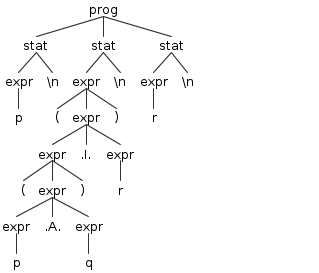
\includegraphics[scale=0.9]{1.png}
	\caption{Gerada com o comando \texttt{\$ java org.antlr.v4.gui.TestRig Expr prog -gui input}, onde \texttt{input} é o arquivo com a entrada (\textbackslash entradas\textbackslash invalidas\textbackslash 8.txt)}
\end{figure}

\subsection{Implementação}

O arquivo EvalVisitor foi criado por nós e nele estão definidas as regras de expansão do Tableau. Atacamos o problema da seguinte forma:

Usamos o ANTLR como base principal do nosso trabalho. A partir dos pedidos da ferramenta, criamos nossa gramática, definida no arquivo \textbf{Expr.g4}. Ele gera os arquivos necessários para o reconhecimento da linguagem. Os arquivos gerados tem a forma Expr*.java.

A ferramenta cria a árvore com os componentes do analisador léxico derivados de gramática. Ele faz o ExprBaseVisitor que define algumas funções que serão executadas quando visitamos alguma estrutura na árvore gerada por ele. Um exemplo disso é o \textbf{Progrule}, que executa o código quando visitamos a estrutura raiz da nossa gramática (visitProgrule).

Cada estrutura de \textbf{expr} dessa árvore possui um valor associado no \textit{ParseTreeProperty} VALORES (é uma estrutura que associa algo a um nó da árvore) que pode ser \textbf{T} (true) ou \textbf{F} (false).

Todas as estruturas \textbf{expr} foram colocadas em uma pilha. Todas as premissas \textbf{expr} foram valoradas como \textbf{T} e a conclusão $B$ como \textbf{F}. O valor da estrutura desempilhada foi devolvido para a saída.

De acordo com a estrutura visitada (recursivamente, com as funções geradas pelo ANTLR) pôde-se definir o que fazer quando:
\begin{itemize}
	\item se entra em situação de operação entre dois elementos ($\to$, $\land$ e $\lor$ - \textbf{visitOp2Atom}).
	\item se entra em situação de negação ($\lnot$ - \textbf{visitOpNot}).
	\item se visita um elemento átomo (\textbf{visitAtom}).
	\item é encontrado um parênteses (\textbf{visitParen}).
	\item é encontrada uma \textbf{expr} comum (\textbf{visitPrintExpr}).
\end{itemize} 

Quando uma expansão $\alpha$ é realizada:
\begin{itemize}
	\item valoramos cada ramo da árvore na estrurura filha em VALORES (do \textbf{ParseTreeProperty}) de acordo com a tabela da expansão $\beta$;
	\item empilhamos a estrutura filha da direita na pilha global;
	\item retornamos o valor da visita na estrutura filha da esquerda.
\end{itemize}

Quando uma oexpansão $\beta$ é realizada:
\begin{itemize}
	\item copiamos a pilha global;
	\item valoramos cada ramo da árvore na estrurura filha em VALORES (do \textbf{ParseTreeProperty}) de acordo com a tabela da expansão $\beta$;
	\item colocamos em uma variável temporária o resultado da visita no ramo esquerdo;
	\item substituimos a pilha pelá cópia anterior;
	\item colocamos em outra variável temporária o resultado da visita no ramo direito ;
	\item devolvemos um AND entre as duas saídas.
\end{itemize}

Quando temos uma operação de negação:
\begin{itemize}
	\item valoramos a única expressão filha como o valor contrário ao valor associado a essa expressão em VALORES;
	\item visitamos a expressão filha.
\end{itemize}

Quando temos um parêntese ou expressão sozinha:
\begin{itemize}
	\item valoramos a expressão filha em VALORES como valor da expressão atual;
	\item visitamos a expressão filha.
\end{itemize}

Quando chegamos em um átomo, verificamos se aquele átomo já possui alguma valor na \textbf{TreeMap} ATOMOS. Caso já possua algum valor nessa \textbf{TreeMap}, o programa verifica se o valor associado àquela estrutura no VALORES e no ATOMOS são diferentes. No caso em que são diferentes então encontramos uma contradição (o que não descarta que a expressão é inválida) e então temos um ramo fechado e retornamos um \textbf{T}. Caso não sejam diferentes então vemos se existe algo na pilha, associando um valor de retorno para a tirada de um elemento da pilha. Ao terminar, se o valor de retorno for \text{F} então encontramos uma situação em que o sequente é inválido, exibimos todos os átomos e seus valores em ATOMOS e encerramos o programa.
 
\end{document}